\documentclass[onecolumn, draftclsnofoot,10pt, compsoc]{IEEEtran}

\usepackage{graphicx}
\graphicspath{{./images/}}

\usepackage{url}
\usepackage{float}
\usepackage{setspace}

\usepackage{listings}

\usepackage{geometry}
\geometry{textheight=9.5in, textwidth=7in}

\usepackage{color}


% COLOR DEFINITIONS FOR CODE LISTINGS
\definecolor{codegreen}{rgb}{0,0.6,0}
\definecolor{codegray}{rgb}{0.5,0.5,0.5}
\definecolor{codepurple}{rgb}{0.58,0,0.82}
\definecolor{backcolour}{rgb}{0.95,0.95,0.92}

\lstdefinestyle{mystyle}{
    backgroundcolor=\color{backcolour},
    commentstyle=\color{codegreen},
    keywordstyle=\color{magenta},
    numberstyle=\tiny\color{codegray},
    stringstyle=\color{codepurple},
    basicstyle=\footnotesize,
    breakatwhitespace=false,
    breaklines=true,
    captionpos=b,
    keepspaces=true,
    numbers=left,
    numbersep=5pt,
    showspaces=false,
    showstringspaces=false,
    showtabs=false,
    tabsize=2
}

\lstset{style=mystyle}



% 1. Fill in these details
\def \CapstoneTeamName{		AKARobotics}
\def \CapstoneTeamNumber{		13}
\def \GroupMemberOne{			Kevin Talik}
\def \GroupMemberTwo{			Anish Asrani}
\def \GroupMemberThree{			Arthur Shing}
\def \CapstoneProjectName{		How to Build an Effective Robot Comedian}
\def \CapstoneSponsorCompany{	Oregon State University}
\def \CapstoneSponsorPerson{		Heather Knight}

% 2. Uncomment the appropriate line below so that the document type works
\def \DocType{		% Problem Statement
				%Requirements Document
				Technology Review
				%Design Document
				%Progress Report
				}

\newcommand{\NameSigPair}[1]{\par
\makebox[2.75in][r]{#1} \hfil 	\makebox[3.25in]{\makebox[2.25in]{\hrulefill} \hfill		\makebox[.75in]{\hrulefill}}
\par\vspace{-12pt} \textit{\tiny\noindent
\makebox[2.75in]{} \hfil		\makebox[3.25in]{\makebox[2.25in][r]{Signature} \hfill	\makebox[.75in][r]{Date}}}}
% 3. If the document is not to be signed, uncomment the RENEWcommand below
%\renewcommand{\NameSigPair}[1]{#1}

%%%%%%%%%%%%%%%%%%%%%%%%%%%%%%%%%%%%%%%
\begin{document}
\begin{titlepage}
    \pagenumbering{gobble}
    \begin{singlespace}
    	% \includegraphics[height=4cm]{coe_v_spot1}
        \hfill
        % 4. If you have a logo, use this includegraphics command to put it on the coversheet.
        %\includegraphics[height=4cm]{CompanyLogo}
        \par\vspace{.2in}
        \centering
        \scshape{
            \huge CS Capstone \DocType \par
            {\large\today}\par
            \vspace{.5in}
            \textbf{\Huge\CapstoneProjectName}\par
            \vfill
            {\large Prepared for}\par
            \Huge \CapstoneSponsorCompany\par
            \vspace{5pt}
            {\Large\NameSigPair{\CapstoneSponsorPerson}\par}
            {\large Prepared by }\par
            Group\CapstoneTeamNumber\par
            % 5. comment out the line below this one if you do not wish to name your team
            \CapstoneTeamName\par
            \vspace{5pt}
            {\Large
                \NameSigPair{\GroupMemberOne}\par
                \NameSigPair{\GroupMemberTwo}\par
                \NameSigPair{\GroupMemberThree}\par
            }
						\vspace{20pt}
        }
        \begin{abstract}
        % 6. Fill in your abstract
        % TODO: Abstract
				This document is a Technology Review written by Arthur Shing of Capstone Group 13, for the research project "How to Create an Effective Robot Comedian" for Heather Knight.
				This document covers an introduction of Shing's roles in the project.
				It also covers topics the group considered for research questions.
				These topics include the effectiveness of different genres, multiple parties, and character.
				This document also reviews different technology that could be used for the robot and its development.
				These include the RoboThespian, the Pepper robot, and the NAO robot.
				Additionally, the development environments considered are the C++ SDK, the Python SDK, and the Choregraphe environment for the NAO robot. 

        \end{abstract}
    \end{singlespace}
\end{titlepage}
\newpage
\pagenumbering{arabic}
\tableofcontents
% 7. uncomment this (if applicable). Consider adding a page break.
%\listoffigures
%\listoftables
\clearpage

% 8. now you write!


\section{Introduction}

This is a tech review for Group 13, written by Arthur Shing, for the project "How to Create an Effective Robot Comedian".
This project is a research project that intends to extend on research done in the field of Human-Robot Interaction.
Our end goal for this project is to create an effective robot comedian that can perform in front of a live audience.
In seeking to create an effective comedian, we hypothesize that comedy scripts with greater degrees of (1) crowdwork, (2) character, and (3) adaptiveness, will create more effective comedy, and have a more positive response from the audience.

\subsection{Role}
As for my own role in this project, I am focusing on (2) the effectiveness of coherent character in comedy.
This entails the creation of comedic scripts with varying degrees of character coherency.

\subsection{Technologies and Research Design}
In the following sections, I will explore the options and choices we had for alternative topics for our second research question on (2) character, robots, and SDKs and environments. Unlike the technology used for the other two research questions of (1) crowd work and (3) adaptiveness, implementing character will require fewer pieces of technology. For instance, both of the other variables will require some sort of sensing technology, while the implementation of character will not. Consequently, I had fewer technological features to choose from after research questions were decided. In place of the third piece of technology, I will discuss choices we considered for research questions.


\section{Research Questions}
The three research questions our group has decided on are the effectiveness of (1) crowd work, (2) character, and (3) adaptiveness in comedy. As a research project, these questions may be subject to change in the future. In deciding upon these three topics, various limitations were taken into account. In this section, I will discuss the decision on (2) character, as well as other topics we considered.

\subsection{Comedic Genre as a research topic}
One topic we considered was the effectiveness of different genres of comedy.
This includes genres such as deadpan, black comedy, slapstick, or specialized robot comedy.
The first thing we considered was the feasibility of implementation.
Deadpan comedy would either be the easiest or hardest part of the implementation, depending on the dynamics of the vocal software.
The NAO's software is likely unable to mimic exaggerations in vocal expressions, but its monotonous (although mildly expressive) delivery may give way to a successful deadpan delivery.
Black comedy is likewise feasible, although probably inappropriate for research.
Slapstick humor would be harder to implement, with movement limitations that the NAO robot has.
Similarly, the NAO robot would be limited by its battery life and its tendency to fall over.
Specialized robot comedy is an area of great interest to us.
This genre of comedy might include robot-specific jokes; jokes that only a robot would have the right to make.
For instance, joking about its own programming, motor, or intellectual deficiencies might prove to be effective.


\subsection{Dialogical Comedy as a research topic}
Another topic we considered was the effectiveness of two parties in stand-up comedy.
In previous tests done by Heather Knight, it was found that a robot by itself could only maintain the attention of a human audience for 2-3 minutes \cite{OneNote:Anish}.
However, with a human interacting with the robot, this time could be extended to twice or three times as long.
Additionally, studies and research could be taken from ventriloquism.
One example of a successful implementation of a robot comedian in tandem with a stand-up comedian in popular culture is Geoff Peterson from The Late Late Show with Craig Ferguson \cite{GeoffPeterson}.
Peterson acted as a sidekick to Ferguson, and although he had an actual voice actor behind the scenes, Peterson could serve as an example of a goal for this topic.
As for implementation on the NAO bot, most of the dialogue would be prescripted with lengths of time between each line for the human to speak.
Another option would be for the human to hold a remote that activates the robot's next line, although this would seem much more scripted.


\subsection{Character as a research topic}
The effectiveness of character design was also a topic under consideration.
In much of early previous work on robot comedy, jokes were simply read off one at a time, resulting in a rigid, static comedic structure \cite{RobotsMakeThings:2008}.
Stand-up comedy, however, seems to thrive off of the buildup before each punchline, as well as the quirkiness of the comedian.
Implementation of this may include writing scripts with varying degrees of character.
Character might involve nonverbal gestures, expressivity, and consistency.
For instance, a script with a high degree of character may mean more pronounced, expressive motions, as well as stronger expressive language.
A script with a moderate degree of character may only include expressive language, or might even employ morose language to portray a different type of character.
On the other hand, a script with a low degree of character may simply ramble off jokes, or speak with a minimal amount of non-verbal language.

\subsection{Discussion of Research Topic Ideas}
Overall, we found that the discussion of character as a research topic might prove to be the more fruitful endeavor.
Additionally, aspects of comedic genre could be incorporated into the topic as a subtopic or stretch goal, seeing that certain genres of comedy necessitate certain comedians.
For instance, robot-specific comedy may require a comedian with a consistently dry or self-deprecating character.
Having the effectiveness of character as a research topic gives us more flexibility in adjusting our research questions in the future, as well as a broader range of ideas to draw from.

\subsection{Conclusion of Research Topic Ideas}
We will research the effectiveness of character implementation in robot comedy.

\section{Robots}
Our project will require a robot as the comedian to conduct testing. This robot ideally has vocal capabilities, as well as gesturing capabilities. The three following robots include both of these capabilities.

\subsection{Robothespian}
The Robothespian has been implemented in Human-Robot Interaction studies in the past.
It is a humanoid, life-sized robot designed for human interaction in public.
It was used to great success in stand-up comedy performance study done by Katevas et. al \cite{KatevasRobot:2014}.
Additionally, it has been used in other theatrical contexts \cite{Spillikin} to some success.
The Robothespian is constructed by Engineering Arts, and comes with a touchscreen kiosk for the user that can be used to trigger content, view sensors, and actively engage or control the robot.
For the most part, the Robothespian uses predefined timed animations in its performances through its stock software \cite{KatevasRobot:2014}.
However, its responsiveness can be optimized in a Python IDE that is provided by Engineering Arts.
The Robothespian stands at a height of roughly 6\", and weighs 97 lbs including a floor base.
The robot also features pneumatic and DC servo motor actuators for the upper body, upper limbs, and head, including jaw actuation and distinct fingers.
It also has a starting price of \pounds59000 \cite{EngineeredArts}.


\subsection{Pepper}
The Pepper robot is a small humanoid robot that was built to perceive and respond to emotions.
Designed by Aldebaran Robotics, the Pepper bot was created to interact as natural and intuitive as possible.
It includes 4 directional microphones on its head, as well as two HD and one 3D camera to locate and identify emotions in voices and faces.
It also comes with six laser sensors, three obstacle detectors, and two ultrasound sensors.
The Pepper robot has also had experience in stage work and has been used in Japan to mild success \cite{PepperVid}.
It specializes in socializing and reacting to perceived emotions.
The robot also comes with a tablet on its chest to supplement human interactivity.
The Pepper weighs in at 62 lbs.
It has a starting price of \$25,000. However, when it was first released, it had a starting price of \$2,000 with a \$300 monthly maintenance fee.
A Pepper SDK for Android was released just this year. \cite{PepperBot}

\subsection{NAO robot}
The NAO robot is a humanoid robot featuring upper and lower body joints.
Also designed by Aldebaran Robotics, it has 25 degrees of freedom and multiple sensors for perceiving the environment.
These include 4 directional microphones, as well as two HD cameras for vocal and facial recognition.
The NAO robot was created to be extremely customizable.
It has a small frame, weighing 9.5 lbs.
It has been previously used to study Human-Robot Interaction and comedy by Knight et al. \cite{KnightSavvy:2011}.
The robot can be programmed through a software produced by Aldebaran Robotics, called Choregraphe.
It has a starting price of \$9,500 \cite{BuyNAO}. \cite{NAORobot}

\subsection{Discussion of Robots}
The NAO Robot is the most accessible to us, as our client already owns one.
The Robothespian and Pepper robot have also only recently launched SDKs for development.
This led us to be wary of possible bugs and issues that have not yet been addressed in development.
Our client is also familiar with the development environment for the NAO robot, which will make learning it an easier process.
In addition, the Robothespian and Pepper robot are priced much higher and lack lower body mobility.
The lower body mobility of the NAO robot may benefit from using non-verbal gestural cues that cannot be done on the other two robots.
These gestures may increase the effectiveness of our comedy \cite{KnightEightLessons:2011}.
The Robothespian and Pepper Robot are also significantly heavier than the tiny NAO robot, which may impact our efficiency with hands-on programming and transporting the robot.

\subsection{Conclusion of Robot Choice}
We decided to use the NAO Robot for our project, based on accessibility and efficiency.

\section{SDKs and Environments}
The NAO Robot can be programmed in several different ways and comes with several different SDKs. It uses an API called NAOqi that is available in eight different languages. However, only C++ and Python are supported on the robot, while the others are only supported on the computer for remote access \cite{NAOSDK:Overview}.

\subsection{C++}
The C++ framework is the most complete one, and allows a developer to write real-time code at high speeds.
The developer can access specialized proxies, which are optimized and give direct access to existing methods.
These proxies also provide compile-time type checking.
The following is an example of specialized proxy usage.

\begin{lstlisting}[language=C++]
	#include <alproxies/altexttospeechproxy.h>

	const std::string phraseToSay = "Hello world";
	AL::ALTextToSpeechProxy tts("nao.local" , 9559);
	tts.say("Hello world");
\end{lstlisting}

In addition to these optimized proxies, generic proxies can also be used.
With these, methods must be specified by the developer, which may be more prone to err.
These are slower than specialized proxies but can adapt to any module.
This includes user-created modules. User-created method names cannot clash with names bound by ALModule methods.
The following is an example of generic proxy usage. \cite{NAOSDK:C++}

\begin{lstlisting}[language=C++]
	#include <alcommon/alproxy.h>

	const std::string phraseToSay = "Hello world";
	AL::ALProxy proxy("ALTextToSpeech", "nao.local", 9559);
	proxy.callVoid("say", phraseToSay);


	// Or, if the method returns something, you
	// must use a template parameter
	bool ping = proxy.call<bool>("ping");
\end{lstlisting}

Movement programmed in C++ is done by calling the angleInterpolation method under the ALMotionProxy module.
This is used by creating an ALValue::array of target angles and times, and passing them into the method.
The following is an example of using angleInterpolation to move the NAO robot's head.
\begin{lstlisting}[language=C++]
	/**
	* Copyright (c) 2011 Aldebaran Robotics. All Rights Reserved
	*/
	#include <iostream>
	#include <alerror/alerror.h>
	#include <alproxies/almotionproxy.h>

	int main(int argc, char* argv[]) {
		const AL::ALValue jointName = "HeadYaw";
    AL::ALMotionProxy motion(argv[1], 9559);
	 	/** Set the target angle list, in radians. */
    AL::ALValue targetAngles = AL::ALValue::array(-1.5f, 1.5f, 0.0f);
    /** Set the corresponding time lists, in seconds. */
    AL::ALValue targetTimes = AL::ALValue::array(3.0f, 6.0f, 9.0f);
    /** Specify that the desired angles are absolute. */
    bool isAbsolute = true;
    /** Call the angle interpolation method. The joint will reach the
    * desired angles at the desired times.
    */
    motion.angleInterpolation(jointName, targetAngles, targetTimes, isAbsolute);
  	exit(0);
	}

\end{lstlisting}



\subsection{Python}
The Python framework is the second most complete, and allows a developer to run embedded code.
Unlike C++, Python does not have two different kinds of proxies.
However, methods can be directly accessed once an ALProxy is set to a module.
The Python API allows a developer to use all of the C++ API from a remote machine.
We can infer that this includes user-created modules.
Programming movement in Python is also done by calling the angleInterpolation method under the ALMotion proxy.
Unlike C++, Python does not require the usage of AL::ALValue::array, and uses its built-in lists.
The following is an example of moving the NAO robot's knee in Python. \cite{NAOSDK:Python}
\begin{lstlisting}[language=Python]
	import sys
	import math
	from naoqi import ALProxy

	def main(robotIP):
    motionProxy = ALProxy("ALMotion", robotIP, 9559)
    # KneePitch angleInterpolation
    # Without Whole Body balancer, foot will fall down
    names      = ["LKneePitch", "RKneePitch"]
    angleLists = [ [0.0, 40.0*math.pi/180.0], [0.0, 40.0*math.pi/180.0]]
    timeLists  = [ [5.0, 10.0], [5.0, 10.0]]
    isAbsolute = True
    motionProxy.angleInterpolation(names, angleLists, timeLists, isAbsolute)

	if __name__ == "__main__":
    robotIp = "127.0.0.1"
    main(robotIp)

\end{lstlisting}

\subsection{Choregraphe}
Choregraphe is a multi-platform desktop application that is designed to create and test animations and behaviors.
Unlike an SDK, Choregraphe allows for development with significantly less coding involved.
All of the NAOqi API is accessible in Choregraphe, and animations can be done in an intuitive way.
Each joint of the NAO robot can be virtually manipulated in a control console. Figure \ref{fig:choregraphe-movement} shows the ways that the left arm of the robot might be manipulated in the console.
These manipulations require no coding and allow for quick and intuitive viewing of movement options.

\begin{figure}[H]
	\centering
	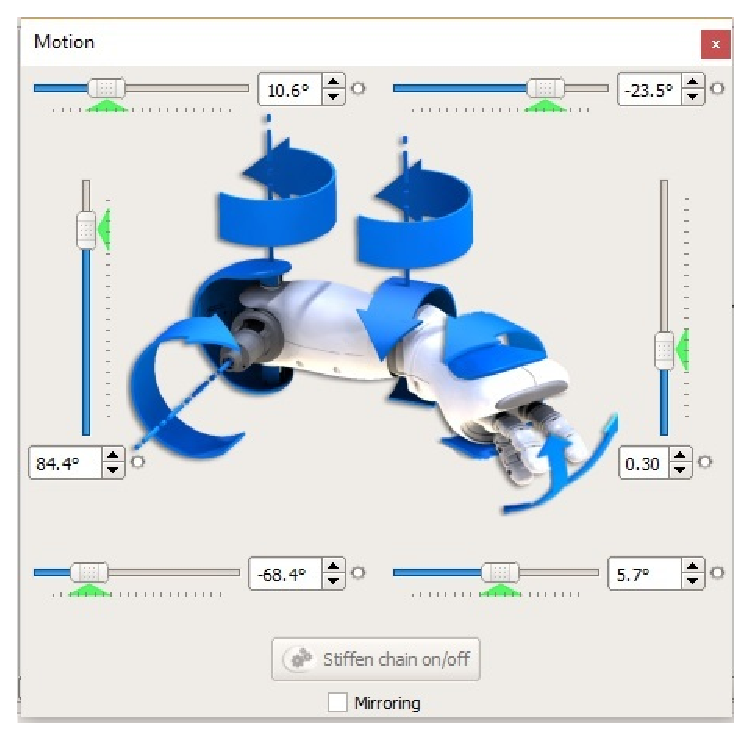
\includegraphics[width=0.5\textwidth]{choregraphe-movement}
	\caption{The motion box in Choregraphe allowing for joint manipulation in the left arm.}
	\label{fig:choregraphe-movement}
\end{figure}

Choregraphe can also connect to an actual or virtual NAO robot as shown in Figure \ref{fig:choregraphe-robot}, allowing programs to be run on the spot.

\begin{figure}[H]
	\centering
	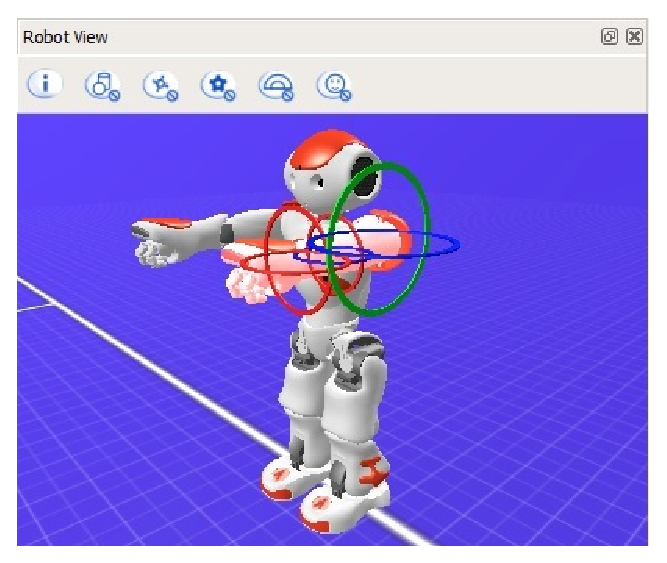
\includegraphics[width=0.5\textwidth]{choregraphe-robot}
	\caption{The virtual robot in Choregraphe. In this image, the left arm can be manipulated.}
	\label{fig:choregraphe-robot}
\end{figure}

Animations can also be created in tandem with vocalizations using a timeline feature, as shown in Figure \ref{fig:choregraphe-timeline}. This feature allows a developer to choose the frames at which the NAO robot will position itself, as well as the words that will be spoken while doing so. \cite{NAOSDK:Choregraphe}

\begin{figure}[H]
	\centering
	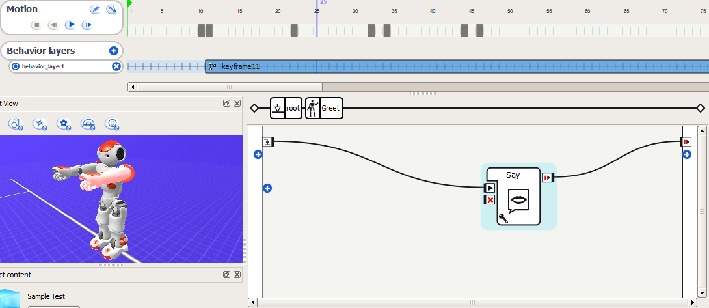
\includegraphics{choregraphe-timeline}
	\caption{The Choregraphe environment. In this image, the timeline is being manipulated for animations along with vocalizations.}
	\label{fig:choregraphe-timeline}
\end{figure}

\subsection{Discussion of SDKs and Environments}
While the C++ and Python SDKs are comprehensive and well made, for my purposes, animations and dynamic actions are a greater focal point.
Because of this, Choregraphe seems like the ideal environment for the research question of the effectiveness of character.
As most tests will involve predetermined scripts and little sensor usage, movement will be a vital part of conveying certain character traits. This will be most efficiently done in Choregraphe.

\subsection{Conclusion of SDK and Environment Choice}
For our purposes, Choregraphe will be used to program the robot.








\bibliographystyle{IEEEtran}
\bibliography{refs}

\end{document}
